% MODIFICATION IMPLEMENTATION
\chapter{3 Implementa��o da modifica��o}

% 3.a OUTPUTS
\section{a. Sa�das}


% 1 Updated Test Plans and Procedures
\subsection{1 Testes planos e procedimentos atualizados}
	Ser� utilizado testes unit�rios com alta cobertura de c�digo, testes de integra��o e testes de interface.
	
	\subsection{An�lise detalhada dos relat�rios}
	
	A imagem a seguir mostra uma parte da realiza��o da migra��o do front end para Vue js
	\begin{figure}
		\centering
		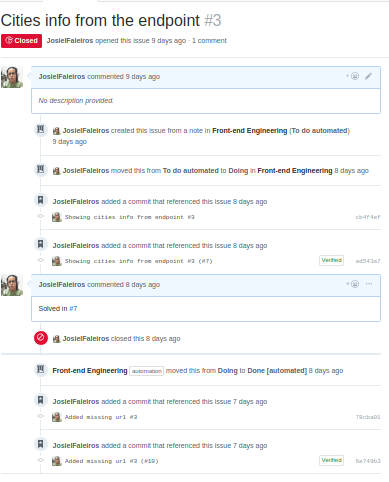
\includegraphics[width=0.7\linewidth]{images/detail-vue-migration}
		\caption{Migra��o para Vue js}
		\label{fig:migracao-front-end}	
	\end{figure}

\newpage

% 2 Updated documentation
\subsection{2 Documenta��o atualizada}
	O mecanismo de issues do github ser� utilizado.

% 3 Modified source code
\subsection{3 C�digo fonte modificado}
	Front end:
		https://github.com/JosielFaleiros/gulosoo-front-end
		
	Back end:
		https://github.com/JosielFaleiros/gulosoo-back-end

	Documento de manuten��o:
		https://github.com/manutencao-software-utfpr/manutencao-software		
		
% 4 Test reporting
\subsection{4 Relat�rios do teste}

\begin{figure}
	\centering
	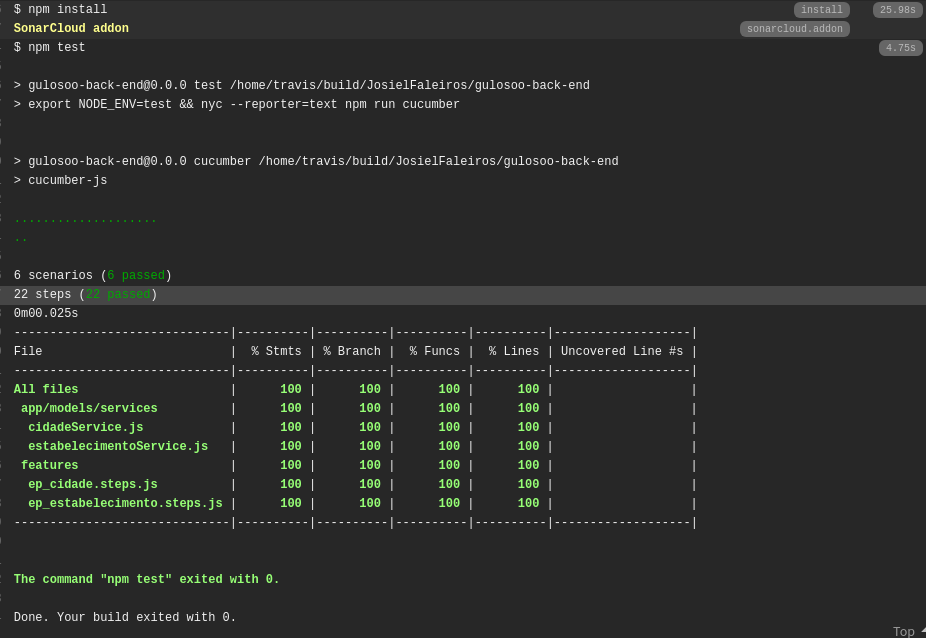
\includegraphics[width=0.7\linewidth]{images/test_report_back-end}
	\caption{Testes Unit�rios}
	\label{fig:reporbgtest}
\end{figure}

\begin{figure}
	\centering
	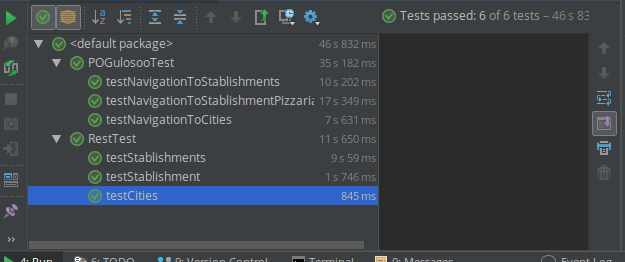
\includegraphics[width=0.7\linewidth]{images/test_report_front-integration}
	\caption{Testes de interface e integra��o}
	\label{fig:reporbgtest}
\end{figure}

\pagebreak

% 5 Measures
\subsection{5 Medi��es}
Estando os testes definidos, � poss�vel a partir de seus resultados entender e as modifica��es levaram a resultados esperados.

